\chapter{Réserves en IARD}
\section{But et motivation}
Un des rôles de l'assurance IARD corporatifs est l'évaluation des provisions actuarielles (réserve).

Contrairement à l'assurance vie, les réserves IARD sont définies par l'Autorité des Marchés Financiers comme :
\begin{quotation}
Le processus d'évaluation du montant total nécessaire pour acquitter tous les paiements futurs associés aux sinistres déjà survenus en date d'évaluation (ex. au 31 décembre).
\end{quotation}

Cette évaluation est très sérieuse, car les réserves IARD représentent $\sim$ 75 \% du passif total de ces assureurs, leurs valeurs affectent directement le profit de la compagnie.

Pour cette raison l'\textit{AMF} requiert notamment que les réserves soient signées par l'actuaire désigné, qui doit obligatoirement être \emph{fellow} de la \emph{CAS} et de l'\emph{ICA}.

Bien que les réserves doivent être déposées à l'AMF au 31 décembre de chaque année, plusieurs assureurs les réévaluent au trimestre ou même au mois.

\subsection*{Remarques}
\begin{enumerate}
\item Habituellement, les réserves IARD sont évaluées par ligne d'affaires. (Assurance auto, habitation, bien commercial, RC entreprise, ferme, aviation, ...)
\\
Ligne d'affaires = produits que l'assureur vend
\item Il est très important de bien évaluer le niveau des réserves IARD
	\begin{itemize}
	\item[a)] Si les réserves sont sous-évaluées:
		\begin{itemize}
		\item On surévalue la santé financière de la compagnie
		\item On expose la compagnie au risque de défaut sur ses paiements futurs
		\item On expose l'assureur à la ruine
		\end{itemize}
	\item[b)] Si les réserves sont surévaluées
		\begin{itemize}
		\item Les dépenses sont plus élevées
		\item Le profit est diminué
		\item Le montant d'impôt à payer est diminué
		\item Le surplus est diminué
		\item La valeur de la compagnie est moindre, donc la valeur de l'action est sous-évaluée.
\end{itemize}				
	\end{itemize}
\end{enumerate}

\section{Définitions}

\subsection*{Différence entre les réserves vie et IARD}
\subsubsection*{Réserves vie}
\begin{align*}
VP_{@u}\Big(\text{Prestations à payer pour les sinistres futurs} \Big) - VP_{@u}\Big(\text{Primes futures à recevoir} \Big)
\end{align*}
\subsubsection*{Réserves IARD}

\begin{align*}
\sum \Bigg( \text{Prestations à payer pour le développement sur les dossiers ouverts en u} \Bigg) - 0
\end{align*}

\subsubsection*{Conséquence}
En IARD, \textbf{LA} problématique derrière l'évaluation des réserves est surtout la modélisation mathématique du développement.


\subsection*{a) Dossier de sinistre (Claim file)}
Dès qu'un sinistre est déclaré à l'assureur, celui-ci ouvre un \textit{dossier} dans son système informatique. Une réclamation correspond à une ouverture d'un dossier. Ce dossier contient plusieurs informations sur la réclamation, tel que
\begin{itemize}
\item La date de perte
\item La date de réclamation
\item Le montant et date de chaque paiement
\item Des informations qualitatives
\end{itemize}

\subsection*{b) Case reserves (réserves automatiques)}
Une estimation des coûts totaux associés à un dossier de sinistres. Cette estimation est faite dès l'ouverture du dossier.

\subsection*{c) Gross IBNR (Incurred but not reported)}

Comporte quatre composantes :
\begin{itemize}
\item[96 \%] Total des provisions pour le développement des sinistres déjà ouverts
\item[1 \%] Les provisions pour dossiers fermés pouvant rouvrir
\item[1 \%] Les provisions pour sinistres encourus, mais non rapportés
\item[1 \%] Les provisions pour les sinistres rapportés, mais non codifiés dans le système informatique.
\end{itemize}

\subsection*{d) Réserve totale}

Réserve totale = Case reserve (10 \%) + Gross IBNR (90 \%)

\subsection*{e) Développement}

Changement temporel de la somme des paiements faits par l'assureur pour tous ses assurés.

\subsection*{f) Paid age-to-age}

Le développement entre deux dates données.

\subsection*{g) Age-to-ultimate development}
Développement des sinistres qui ont atteint un âge donné jusqu'à l'ultime moment où ces dossiers sont fermés.

\subsection*{h) Loss development factor $(LDF_{j-1, j})$}
Aussi appeler le \emph{Paid loss development factor}.
\begin{align*}
LDF_{j-1, j} & = \frac{\text{Somme des paiements faits par l'assureur sur tous les dossiers de sinistres à t = j}}{\text{Somme des paiements fait par l'assureur sur tous les dossiers des sinistres à t = j - 1}}
\end{align*}

\subsection*{i) Sinistres en suspend (SS)}
Somme des \emph{cases reserves} révisées pour tous les sinistres qui ne sont pas encore fermés à une date donnée.

\subsection*{j) Sinistres payés (SP)}
Somme des montants d'indemnités payés aux réclamants à une date donnée.

Inclus les frais de règlement aussi.

\subsection*{k) Sinistres encourus (SE)}
Somme des montants engendrés par des sinistres qui ont donné (SP), ou qui donneront (SS) lieu à des paiements d'indemnités à une date donnée.
$$ SE = SP + SS $$

\subsection*{l) Incurred loss development factor $(ILDF_{j-1, j})$}

\begin{align*}
ILDF_{j-1, j} &= \frac{\sum SE_{@j}}{\sum SE_{@j-1}} \\
&= \frac{C_j}{C_{j-1}} \\
&= \frac{\text{Encouru cumulatif à $t = j$}}{\text{Encouru cumulatif à $t = j-1$}}
\end{align*}

\subsection*{m) Notations en triangles cumulatifs ($\triangleleft$)}
On débute par un exemple pour illustrer la présentation des données.

Ex.:\\

\begin{center}
\begin{tabular}{|c|c|c|c|c|c|}
  \hline
   AA/âge & 12 mois & 24 mois & 36 mois & 48 mois & 60 mois \\
  \hline
  2012 & $C_{2012, 12}$ & $C_{2012, 24}$ & $C_{2012, 36}$ & $C_{2012, 48}$ & $C_{2012, 60}$\\
  2013 & $C_{2013, 12}$ & $C_{2013, 24}$ & $C_{2013, 36}$ & $C_{2013, 48}$ & ?\\
  2014 & $C_{2014, 12}$ & $C_{2014, 24}$ & $C_{2014, 36}$ & ? & ?\\ 
  2015 & $C_{2015, 12}$ & $C_{2012, 24}$ & ? & ? & ? \\
  2016 & $C_{2016, 12}$ & ? & ? & ? & ?\\ 
  \hline
\end{tabular}
\end{center}

Où AA est l'année d'accident qui correspond à l'année de la date de survenance du sinistre.

\subsection*{Notation académique}
Afin d'alléger la notation, on utilise la notation simplifiée suivante:

\begin{center}
\begin{tabular}{|c|c|c|c|c|c|}
  \hline
   $AA_i$/$\widehat{a}ge_j$ & 1 & 2 & 3 & 4 & 5 \\
  \hline
  1 & $C_{1, 1}$ & $C_{1, 2}$ & $C_{1, 3}$ & $C_{1, 4}$ & $C_{1, 5}$\\
  2 & $C_{2, 1}$ & $C_{2, 2}$ & $C_{2, 3}$ & $C_{2, 4}$ & ?\\
  3 & $C_{3, 1}$ & $C_{3, 2}$ & $C_{3, 3}$ & ? & ?\\ 
  4 & $C_{4, 1}$ & $C_{4, 2}$ & ? & ? & ? \\
  5 & $C_{5, 1}$ & ? & ? & ? & ?\\ 
  \hline
\end{tabular}
\end{center}

Ainsi $C_{i,j}$ est le montant total payé par l'assureur pour tous les sinistres survenus lors de l'année i ($AA_i$)  et développés pendant j années ($\widehat{a}ge_j$).

\section{Méthode du Chain-Ladder}
Cette méthode est la plus employée en pratique. Elle suppose
$$ C_{i,j+1} = C_{i,j} \times LDF_j $$
Si on dispose d'un triangle de n années de données cumulatives, alors la méthode de C-L revient à effectuer n-1 régressions linéaires simples sans ordonnées à l'origine.

Ainsi, par la théorie de la régression linéaire simple, on peut montrer que

$$ \widehat{LDF}_j = \frac{\sum_{i=1}^{n-j} C_{i, j + 1}}{\sum_{i=1}^{n-j} C_{i,j}} ; \forall j = 1,2,...,n-1$$

Exemple:

\begin{center}
\begin{tabular}{|c|c|c|c|c|c|}
  \hline
   $AA_i$/$\widehat{a}ge_j$ & 1 & 2 & 3 & 4 & 5 \\
  \hline
  1 & 100 & 150 & 175 & 180 & 200 \\
  2 & 110 & 168 & 192 & 205 & ?\\
  3 & 115 & 169 & 202 & ? & ?\\ 
  4 & 125 & 185 & ? & ? & ? \\
  5 & 150 & ? & ? & ? & ?\\ 
  \hline
\end{tabular}
\end{center}
On obtient les LDF suivants:
\begin{align*}
\widehat{LDF}_4 &= \frac{200}{180} = 1.11 \\
\widehat{LDF}_3 &= \frac{180+205}{175+192} = 1.049046 \\
\widehat{LDF}_2 &= \frac{175+192+202}{150+168+169} = 1.168738 \\
\widehat{LDF}_1 &= \frac{150+168+169+185}{100+110+115+125} = 1.493
\end{align*}

Selon C-L
\begin{align*}
\widehat{C}_{2,5} &= C_{2,4} \times \widehat{LDF}_4 = 205 \times 1.111 = 227.77 \\
\widehat{C}_{3,4} &= C_{3,3} \times \widehat{LDF}_3 = 202 \times 1.049046 = 211.9074\\
\widehat{C}_{3,5} &= \widehat{C}_{3,4} \times \widehat{LDF}_4 \\
&= \Bigg( C_{3,3} \times \widehat{LDF}_3 \Bigg) \times \widehat{LDF}_4 \\
&= 202 \times 1.04906 \times 1.111 \\
&= 235.4526 \\
\widehat{C}_{4,5} &= \widehat{C}_{4,2} \times \widehat{LDF}_2 \times \widehat{LDF}_3 \times \widehat{LDF}_4 \\
\end{align*}
On note une forme de récurrence dans les développements. 

Cette forme de récurrence nous permet d'estimer les informations dans le triangle de donnée précédent,

\begin{center}
\begin{tabular}{|c|c|c|c|c|c|}
  \hline
   $AA_i$/$\widehat{a}ge_j$ & 1 & 2 & 3 & 4 & 5 \\
  \hline
  1 & 100 & 150 & 175 & 180 & 200 \\
  2 & 110 & 168 & 192 & 205 & 227.77\\
  3 & 115 & 169 & 202 & 211.9074 & 235.4526\\ 
  4 & 125 & 185 & 216.21653 & 226.8211 & 251.7714 \\
  5 & 150 & 223.95 & 261.7389 & 274.57612 & 304.7794\\ 
  \hline
\end{tabular}
\end{center}
\subsection*{En résumé, selon C-L}
\begin{equation}
\label{eq:CL}
\widehat{C}_{i,n} = C_{i,n-i+1} \times LDF_{n-i+1} \times ... \times LDF_{n-1}; i =1,2,...n
\end{equation}

\subsection*{Réserve selon C-L}
La réserve C-L pour l'AA i est notée $\widehat{R_i}$ et correspond à la différence entre les sinistres \textit{ultimes} ($\widehat{C}_{i,n}$) et les sinistres payés en date d'évaluation ($\widehat{C}_{i,n-i+1}$).
\begin{equation}
\widehat{R_i} = \widehat{C}_{i,n} - \widehat{C}_{i,n-i+1}
\end{equation}

De notre exemple précédant, on obtient 

\begin{center}
\begin{tabular}{|c|c|c|c|}
  \hline
   i & $ \widehat{C}_{i,n} $ & $\widehat{C}_{i,n-i+1}$ & $\widehat{R}_i$  \\
  \hline
  1 & 200 & 200 & 0 \\
  2 & 227.77 & 205 & 22.78 \\
  3 & 235.45 & 202 & 33.45 \\
  4 & 251.7714 & 185 & 66.7714 \\
  5 & 304.7794 & 150 & 154.7795 \\
  \hline
\end{tabular}
\end{center}
Finalement, la réserve totale inscrite au passif des états financiers est notée $\widehat{R}$ et est telle que
$$ R = \sum_{i=1}^{n} \widehat{R}_i $$
Dans notre exemple, elle correspond à
\begin{align*}
R &= \sum_{i=1}^{n} \widehat{R}_i \\
&= 0 + 22.78 +33.45 + 66.7714 + 154.7795 \\
&=277.7809
\end{align*}

\subsection*{Remarques sur C-L}
\begin{itemize}
\item[1)] C-L suppose que les AA (=lignes du triangle) sont indépendantes.
\item[2)] C-L assume que l'âge des sinistres est la seule variable explicative du développement.
\item[3)] C-L suppose aussi $LDF_{i,j} = LDF_j$, n'est pas fonction de l'AA i.
\item[4)] Avec Chain-Ladder, la réserve $\widehat{R}_n$ de l'AA la plus récente est sujette à une forte incertitude.
\end{itemize}

\newpage
\section{Méthode de Bornhuetter-Ferguson}

L'objectif de cette méthode est de permettre une meilleure \emph{stabilité} dans l'estimation des réserves $\widehat{R}_i $ pour les AA i les plus récentes.
En d'autres mots, on veut corriger le désavantage principal de Chain-Ladder avec Bornhuetter-Ferguson .

\subsection*{Trois grandes étapes:}
\begin{enumerate}
\item Estimation des sinistres ultimes $\Rightarrow \widehat{C}_{i,n}$ \newline
En pratique, on utilise un taux de sinistre \emph{(Loss ratio)} qui est \textit{assumé} comme \textit{connu}, et on multiplie ce \emph{loss ratio} par les primes acquises ($PA_i$). Soit,
$$ \widehat{C}_{i,n}^{B-F} = PA_i \times LR_i \text{ ; } i = 1,2,...,n$$ 
Où $LR_i$ est un avis d'expert.

\item Calcul des facteurs de développements ($\widehat{LDF}_i$) \newline
Avec la même méthode/formule qu'avec la Chain-ladder
$$ \widehat{LDF}_j = \frac{\sum_{i = 1}^{n-1} C_{i, j+1}}{\sum_{i = 1}^{n-1} C_{i, j}}$$

\item Calcul de la réserve \newline
On débute avec la définition de $\widehat{R}_i^{C-L}$,
\begin{align*}
\widehat{R}_i &= \widehat{C}_{i,n} - C_{i, n-i+1} \\
&= \widehat{C}_{i,n} \times \Bigg( 1 - \frac{C_{i, n-i+1}}{\widehat{C}_{i,n}}\Bigg) \\
&\overset{(\ref{eq:CL})}{=} \widehat{C}_{i,n} \times \Bigg( 1 - \frac{C_{i, n-i+1}}{\widehat{C}_{i,n -i + 1} \times \prod_{j = n - i + 1}^{n- 1} \widehat{LDF}_j}\Bigg)  \\
\end{align*}
\begin{equation}
\label{eq:BFmet}
\widehat{R}_i^{B-F} = \widehat{C}_{i,n}^{B-F} \times \Bigg( 1 - \frac{1}{\prod_{j = n - i + 1}^{n- 1} \widehat{LDF}_j}\Bigg)  \\
\end{equation}
\end{enumerate}

\subsection*{Exemple}

\begin{center}

\begin{tabular}{|c|c|c|c|c|}
  \hline
   AA & PA & LR & $\widehat{C}_{i,n}^{BF} = U$ & $1 - \frac{1}{\prod LDF_i}$  \\
  \hline
  2010 & 330 & 0.6 & 198 & 0 \\
  2011 & 350 & 0.65 & 228 & 0.1 \\
  2012 & 365 & 0.7 & 256 & 0.14 \\
  2013 & 385 & 0.75 & 289 & 0.26 \\
  2014 & 400 & 0.8 & 320 & 0.51 \\
  \hline
\end{tabular}
\end{center}
À l'aide de l'équation \ref{eq:BFmet}
\begin{align*}
R_1^{B-F} &= \widehat{C}_{1,5}^{BF} \times \Bigg( 1 - \frac{1}{\prod_{j = 5 - 1 + 1}^{5 - 1} \widehat{LDF}_i}\Bigg)  \\
&= \widehat{C}_{1,5}^{BF} \times \Bigg( 1 - \frac{1}{\prod_{j = 5 }^{4} \widehat{LDF}_i}\Bigg)  \\
&= 198 \times 0 \\
&= 0 \\
R_2^{B-F} &= \widehat{C}_{2,5}^{BF} \times \Bigg( 1 - \frac{1}{\prod_{j = 5 - 2 + 1}^{5 - 1} \widehat{LDF}_i}\Bigg)  \\
&= \widehat{C}_{2,5}^{BF} \times \Bigg( 1 - \frac{1}{\widehat{LDF}_4}\Bigg)  \\
&= 228 \times 0.1 \\
&= 22.8 \\
R_3^{B-F} &= \widehat{C}_{3,5}^{BF} \times \Bigg( 1 - \frac{1}{\prod_{j = 5 - 3 + 1}^{5 - 1} \widehat{LDF}_i}\Bigg)  \\
&= \widehat{C}_{3,5}^{BF} \times \Bigg( 1 - \frac{1}{\widehat{LDF}_3\widehat{LDF}_4}\Bigg)  \\
&= 256 \times 0.14 \\
&= 35.84 \\
\end{align*}
\begin{align*}
R_4^{B-F} &= \widehat{C}_{4,5}^{BF} \times \Bigg( 1 - \frac{1}{\prod_{j = 5 - 4 + 1}^{5 - 1} \widehat{LDF}_i}\Bigg)  \\
&= \widehat{C}_{4,5}^{BF} \times \Bigg( 1 - \frac{1}{\widehat{LDF}_2\widehat{LDF}_3\widehat{LDF}_4}\Bigg)  \\
&= 289 \times 0.26 \\
&= 75.14 \\
R_5^{B-F} &= \widehat{C}_{5,5}^{BF} \times \Bigg( 1 - \frac{1}{\prod_{j = 5 - 5 + 1}^{5 - 1} \widehat{LDF}_i}\Bigg)  \\
&= \widehat{C}_{5,5}^{BF} \times \Bigg( 1 - \frac{1}{\widehat{LDF}_1\widehat{LDF}_2\widehat{LDF}_3\widehat{LDF}_4}\Bigg)  \\
&= 320 \times 0.51 \\
&= 163.2 \\
\end{align*}

\begin{center}
\begin{tabular}{|c|c|}
  \hline
   AA & $R_i$  \\
  \hline
  2010 & 0 \\
  2011 & 22.8 \\
  2012 & 35.84 \\
  2013 & 75.14 \\
  2014 & 163.2 \\
  \hline
  \hline
  $\sum_{i = 2010}^{2014} R_i = $   & 296.98 \\
  \hline
\end{tabular}
\end{center}
\subsubsection*{Terminologie}
\begin{itemize}
\item[•] $\frac{1}{\prod_{j = n - i + 1}^{n - 1} \widehat{LDF}_i}$ est appeler le pourcentage des sinistres développés. 
À partir de l'exemple précédant, le pourcentage des sinistres développés de l'année 2011 est de 90 \%.
\item[•] $1 - \frac{1}{\prod_{j = n - i + 1}^{n - 1} \widehat{LDF}_i}$ est appeler le pourcentage des sinistres non développés. 
À partir de l'exemple précédant, le pourcentage des sinistres non développés de l'année 2011 est de 10 \%.
\end{itemize}

\subsection*{Remarques}
\begin{enumerate}
\item L'avantage de Bornhuetter-Ferguson est qu'elle procure une meilleure stabilité dans les réserves $\widehat{R}_i$ des AA i plus récentes.
\item Le désavantage souvent cité de Bornhuetter-Ferguson est l'utilisation de données \emph{externes} ($PA_i$ et $LR_i$) qui peuvent introduire de la \emph{subjectivité}.
\item Dans la méthode de Bornhuetter-Ferguson, c'est un peu comme si on faisait l'hypothèse que l'âge des sinistres n'affecte pas le développement.
\begin{align*}
\bullet B-F &\Rightarrow \widehat{C}_{i,n}^{B-F} = PA_i \times LR_i \equiv a_i + C_{i,n-i+1} \times 0 \\
\bullet C-L &\Rightarrow \widehat{C}_{i,n}^{C-L} = C_{i,n-i+1} \times \Big(\prod_{j=n-i+1}^{n-1} \widehat{LDF}_j \Big) = 0 + C_{i,n-i+1} \times \beta_i \\
\end{align*}
\end{enumerate}


\section{Méthode de Mack}
Bien que la méthode Chain-ladder et la méthode Bornhuetter-Ferguson soient très efficaces pour estimer les réserves espérées, elles ont la limitation de ne pas pouvoir quantifier la variance de ces réserves. La méthode de Mack permet ceci en ajustant un cadre stochastique à la méthode Chain-Ladder.

\subsection*{Trois hypothèses de Mack}
\begin{enumerate}
\item Les AA sont indépendantes, c'est à dire $\lbrace C_{1,1}, ..., C_{1,n} \rbrace \bot \lbrace C_{2,1}, ..., C_{2,n}\rbrace \bot ... $
\item E $\Big[ C_{i, k+1} | C_{i,1}, ..., C_{i,k}\Big] = C_{i,k} \times LDF_k \text{ ; }i = 1, ..., n \text{ et } k = 1, ..., n-1$ 
\item Var $\Big( C_{i, k+1} | C_{i,1}, ..., C_{i,k}\Big) = C_{i,k} \times \sigma_k^2 \text{ ; }i = 1, ..., n \text{ et } k = 1, ..., n-1$ 
\end{enumerate}

\subsection*{Définition}
\begin{itemize}
\item $H_i = \lbrace C_{i,1}, ..., C_{i,n-i+1} \rbrace$: Les données $C_{i,j}$ disponible dans le triangle pour l'AA i.
\item $D = \lbrace C_{i,j} \text{ : } i+j \leq n + 1 \rbrace$: Le triangle de données complet.
\end{itemize}
Sous cette spécification, on peut montrer que le meilleur estimateur de $LDF_j$ est les mêmes qu'avec Chain-Ladder.
\begin{align*}
\widehat{LDF}_j = \frac{\sum_{i = 1}^{n-j}C_{i,j+1}}{\sum_{i = 1}^{n-j}C_{i,j}}
\end{align*}
\subsubsection*{Idée de la preuve précédante}
\begin{align*}
E[C_{i,j} | D] &\overset{H1}{=} E[C_{i,j}|H_i] \\
&= E\Big[ E[C_{i,j}|C_{i,j},...,C_{i,j-1}] \big| H_i \Big] \\
&\overset{H2}{=} E[C_{i,j-1}|H_i] \times LDF_{j-1} \\
&= \text{à appliquer plusieurs fois...} \\
&=C_{i,n-i+1} \times LDF_{n-i+1} \times ... \times LDF_{j-1} \\
\end{align*}
Ce qui coïncide avec Chain-Ladder.

\subsubsection*{Conséquences des hypothèses}

Une première conséquence des hypothèses de Mack est 
\begin{align*}
E[\widehat{LDF}_k|D_k] &\overset{\text{déf}}{=} E \Bigg[ \frac{\sum_{i =1}^{n-k} C_{i,k+1}}{\sum_{i =1}^{n-k} C_{i,k}} \bigg| D_k \Bigg] \\
&= \frac{E[\sum_{i =1}^{n-k} C_{i,k+1} |D_k] }{\sum_{i =1}^{n-k} C_{i,k}} \\
&= \frac{\sum_{i =1}^{n-k} E[ C_{i,k+1} |D_k] }{\sum_{i =1}^{n-k} C_{i,k}} \\
&= \frac{\sum_{i =1}^{n-k} C_{i,k} \times LDF_k }{\sum_{i =1}^{n-k} C_{i,k}} \\
&= \Bigg( \frac{\sum_{i =1}^{n-k} C_{i,k}}{\sum_{i =1}^{n-k} C_{i,k}} \Bigg) \times LDF_k \\
E[\widehat{LDF}_k|D_k] &= LDF_k \text{ (sans biais)}
\end{align*}


De plus, pour $k<j$, on a que
\begin{align*}
E[\widehat{LDF}_k \times \widehat{LDF}_j] &= E \Big[ E[ \widehat{LDF}_k \times \widehat{LDF}_j | D_j]\Big] \\
&= E \Big[ LDF_k \times E[\widehat{LDF}_j |D_j \Big] \\
&= E [ \widehat{LDF}_k ] \times E[\widehat{LDF}_j] \\
\Rightarrow \text{cov}(\widehat{LDF}_k, \widehat{LDF}_j) &= E[\widehat{LDF}_k \times \widehat{LDF}_j] - E [ \widehat{LDF}_k ] \times E[\widehat{LDF}_j] \\
&= 0 \rightarrow \text{(non corrélés)}
\end{align*}

Cette non-corrélation est essentielle, elle permet d'écrire le développement suivant

\begin{align*}
E[\widehat{R}_i] &= E[\widehat{C}_{i,n} - \widehat{C}_{i, n-i+1}] \\
&= E[C_{i,n - i + 1} \times \widehat{LDF}_{n-i+1} \times ... \times \widehat{LDF}_{n-1} - \widehat{C}_{i, n-i+1}] \\
&= C_{i,n - i + 1} E[\widehat{LDF}_{n-i+1} \times ... \times \widehat{LDF}_{n-1}] - \widehat{C}_{i, n-i+1} \\
&= C_{i,n - i + 1} E[\widehat{LDF}_{n-i+1}] \times ... \times E[\widehat{LDF}_{n-1}] - \widehat{C}_{i, n-i+1} \\
&= C_{i,n - i + 1} LDF_{n-i+1} \times ... \times LDF_{n-1} - \widehat{C}_{i, n-i+1} \\
&= R_i
\end{align*}
Sous Mack, $\widehat{R}_i$ est un estimateur sans biais de la réserve de l' AA i.

\subsubsection*{Remarque}
\begin{align*}
E[\widehat{R}] &= E \Big[ \sum_{i=1}^{n} \widehat{R}_i \Big] \\
&= \sum_{i=1}^{n} E \Big[  \widehat{R}_i \Big] \\
&= \sum_{i=1}^{n} R_i \\
&= R \text{  (sans biais)}
\end{align*}

\section*{Estimation de la volatilité (la variance) des réserves}
\subsubsection*{Rappel}
L'hypothèse numéro 3 : Var $\Big( C_{i, j+1} | C_{i,1}, ..., C_{i,j}\Big) = C_{i,j} \times \sigma_j^2$

\subsection*{Proposition de Mack pour estimer $\widehat{\sigma}_j$}
À partir du triangle de données, on peut trouver les relations suivantes:
\begin{align*}
\widehat{LDF}_2 &= \frac{\sum_{i=1}^{3} C_{i,3}}{\sum_{i=1}^{3} C_{i,2}} \\
&= \sum_{i=1}^{3} \Bigg( \frac{C_{i,2}}{\sum_{k=1}^{3}C_{k,2}}\Bigg) \frac{C_{i,3}}{C_{i,2}}
\end{align*}
On observe que les \emph{age to age factor} correspondent à
\begin{align*}
A_{to}A_{1,2} &= \frac{C_{1,3}}{C_{1,2}} \\
A_{to}A_{2,2} &= \frac{C_{2,3}}{C_{2,2}} \\
A_{to}A_{3,2} &= \frac{C_{3,3}}{C_{3,2}} \\
\end{align*}
On peut donc faire la relation entre les \emph{LDF} et les \emph{age to age factor},
\begin{align*}
\widehat{LDF}_2 &= \sum_{i=1}^{3} W_i A_{to}A_{i,2}
\end{align*}
où $ W_i = \frac{C_{i,2}}{\sum_{k=1}^{3}C_{k,2}}$.
\\
Remarque : $\sum_{i=1}^{3} W_i= 1$

\subsubsection*{L'analogue pour $\widehat{\sigma}_2^2$}
\begin{align*}
\widehat{\sigma}_2^2 &= \frac{1}{n-j-1} \sum_{i=1}^{n-j} C_{i,2} \Bigg( \frac{C_{i,3}}{C_{i,2}} - \widehat{LDF}_2\Bigg)^2
\end{align*}
Où $\frac{1}{n-j-1}$ est la correction pour être sans biais et $\frac{C_{i,3}}{C_{i,2}}$ est le \emph{age to age ratio} ($A_{to}A_{i,3}$).

\subsection*{Cas général}
\begin{equation}
\label{eq:est:sigm}
\widehat{\sigma}_j^2 = \frac{1}{n-j-1} \sum_{i=1}^{n-j} C_{i,j} \Bigg( \frac{C_{i,j+1}}{C_{i,j}} - \widehat{LDF}_j\Bigg)^2
\end{equation}

\subsubsection*{Preuve}
\begin{itemize}
\item[I)]\begin{align*}
E \Bigg[ \Bigg( \frac{C_{i,j+1}}{C_{i,j}} - \widehat{LDF}_j \Bigg)^2 \bigg| D_j \Bigg] &= E \Bigg[ \Bigg( \frac{C_{i,j+1}}{C_{i,j}} - LDF_j\Bigg)^2 \Bigg| D_j \Bigg] \\ 
&- 2 E \Bigg[ \Bigg( \frac{C_{i,j+1}}{C_{i,j}} - LDF_j\Bigg) \times (\widehat{LDF}_j - LDF_j) \Bigg| D_j \Bigg] \\
&+ E \Bigg[ \Bigg( \widehat{LDF}_j- LDF_j \Bigg)^2 \Bigg| D_j \Bigg] \\
\end{align*}
\item[II)]\begin{align*}
E \Bigg[ \Bigg( \frac{C_{i,j+1}}{C_{i,j}} - LDF_j\Bigg)^2 \Bigg| D_j \Bigg] &= \text{Var}\Bigg( \frac{C_{i,j+1}}{C_{i,j}} \Bigg|D_j\Bigg) = \frac{\sigma_j^2}{C_{i,j}} \\
E \Bigg[ \Bigg( \frac{C_{i,j+1}}{C_{i,j}} - LDF_j\Bigg) \times (\widehat{LDF}_j - LDF_j) \Bigg| D_j \Bigg]  &= \text{Cov} \Bigg( \frac{C_{i,j_1}}{C_{i,j}}, \widehat{LDF}_j \Bigg|D_j \Bigg) \\
&= \frac{\sigma_j^2}{\sum_{i=1}^{n-j} C_{i,j}} \\
\end{align*}
\item[III)] \begin{align*}
E[\sigma_j^2] = \sigma_j^2 \text{ en substituant II et I}
\end{align*}
\end{itemize}
\bigskip


Par conséquent, l'erreur quadratique moyenne de la réserve pour l'AA i est

\begin{align*}
MSE(\widehat{R}_i) =E \big[ (\widehat{R}_i - R_i)^2 | D \big]
\end{align*}
et est estimée par
\begin{equation}
MSE(\widehat{R}_i) = \widehat{C}_{i,n}^2 \sum_{k = n - i + 1}^{n-1} \frac{\widehat{\sigma}_k^2}{(LDF_k)^2} \Bigg( \frac{1}{\widehat{C}_{i,k}} + \frac{1}{\sum_{j=1}^{n-k}C_{j,k}}\Bigg)
\end{equation}
\subsubsection*{Remarque}
Lorsque k = n - 1, soit le dernier terme de la somme, on a que
\begin{align*}
\widehat{\sigma}_{n-1}^2 &= \frac{1}{n-(n-1)-1} \Bigg( \frac{C_{i,n}}{C_{i,n-1}} - \widehat{LDF}_{n-1}\Bigg)^2
\end{align*}
On note que $\frac{1}{n-(n-1)-1} = \frac{1}{0}$. Cette situation étant problématique, deux solutions ont été proposées:
\begin{itemize}
\item[1)] On pose $\widehat{\sigma}_{n-1}^2 = \widehat{\sigma}_{n-2}^2$
\item[2)] Il est d'usage, en pratique, d'utiliser la forme suivante si $\widehat{\sigma}_{j}^2$ n'est pas complètement plat pour j grand,
\begin{align*}
\widehat{\sigma}_{n-1}^2 &= \text{min} \Bigg( \frac{\widehat{\sigma}_{n-2}^4}{\widehat{\sigma}_{n-3}^2}, \text{min} \Big( \widehat{\sigma}_{n-3}^2, \widehat{\sigma}_{n-2}^2 \Big) \Bigg)
\end{align*}
\end{itemize}

\subsection*{I.C. pour $\widehat{R}_i$}
Deux options fournies par Mack,
\begin{itemize}
\item[1)] On suppose que 
\begin{align*}
R_i \sim N \bigg\lbrace MU_i &= E[\widehat{R}_i]; SIGMA_i^2 = MSE(\widehat{R}_i) \bigg\rbrace \\
\Rightarrow IC^N(\widehat{R}_i) &= \bigg[ \widehat{R}_i - Z_{\frac{\alpha}{2}} \times \sqrt{MSE(\widehat{R}_i)}; \widehat{R}_i + Z_{\frac{\alpha}{2}} \times \sqrt{MSE(\widehat{R}_i)} \bigg]
\end{align*}
\item[2)] On suppose que 
\begin{align*}
R_i \sim LN \Bigg\lbrace MU_i &= \text{ln}(\widehat{R}_i) - \frac{SIGMA_i^2}{2}; SIGMA_i^2 = \text{ln} \Bigg( 1 + \Bigg( \frac{\sqrt{MSE(\widehat{R}_i)}}{\widehat{R_i}}\Bigg)^2 \Bigg) \Bigg\rbrace \\
\Rightarrow IC^{LN}(\widehat{R}_i) &= \Bigg[ e^{MU_i - Z_{\frac{\alpha}{2}} \times \sqrt{SIGMA_i^2}}; e^{MU_i + Z_{\frac{\alpha}{2}} \times \sqrt{SIGMA_i^2}} \Bigg]
\end{align*}
\end{itemize}

\subsection*{MSE et I.C. pour $\widehat{R} = \sum_{i=1}^{n}\widehat{R}_i$}
La volatilité de la réserve totale est donnée par
\begin{align*}
MSE(\widehat{R}) &= E \Big[ (\widehat{R} - R)^2 |D \Big] \\
&= E \Bigg[ \bigg( \sum_{i=2}^{n} \widehat{R}_i -  \sum_{i=2}^{n} R_i)^2\bigg) \Big|D \Bigg] \\
\end{align*}
et est estimée par
\begin{align*}
MSE(\widehat{R}) &= \sum_{i=2}^{n} \Bigg( \widehat{MSE}(\widehat{R}_i) + \widehat{C}_{i,n} \times \Big( \sum_{j = i + 1}^{n} \widehat{C}_{j,n} \Big) \times \sum_{k = n - i + 1}^{n-1} \frac{\frac{2 \widehat{\sigma}_k^2}{\widehat{LDF}_k^2}}{\sum_{j=1}^{n-k} C_{j,k}}  \Bigg)
\end{align*}
Deux options fournies pour I.C.
\begin{itemize}
\item[1)] \begin{align*}
R \sim N \bigg\lbrace MU &= \widehat{R}; SIGMA^2 = MSE(\widehat{R}) \bigg\rbrace \\
\Rightarrow IC^N(\widehat{R}) &= \bigg[ \widehat{R} - Z_{\frac{\alpha}{2}} \times \sqrt{MSE(\widehat{R})}; \widehat{R} + Z_{\frac{\alpha}{2}} \times \sqrt{MSE(\widehat{R})} \bigg]
\end{align*}
\item[2)] \begin{align*}
R \sim LN \Bigg\lbrace MU &= \text{ln} (\widehat{R}) + \frac{SIGMA^2}{2}; SIGMA^2 = \text{ln} \Bigg( 1 + \Bigg( \frac{\sqrt{MSE(\widehat{R}_i)}}{\widehat{R_i}}\Bigg)^2 \Bigg) \Bigg\rbrace \\
\Rightarrow IC^{LN}(\widehat{R}) &= \bigg[ e^{MU - Z_{\frac{\alpha}{2}} \times \sqrt{SIGMA^2}}; e^{MU + Z_{\frac{\alpha}{2}} \times \sqrt{SIGMA^2}} \bigg]
\end{align*}
\end{itemize}

\section{Méthode basée sur les GLM}

Bien que la méthode de Mack introduise la notation de variabilité dans les réserves IARD. Les GLM permettent de faire plus:
\begin{itemize}
\item[1)] Ils ne se limitent pas à la distribution Normale ou Log-Normale, mais admettent toutes les distributions de la famille exponentielle (Normale, Log-Normale, Binomiale, Poisson, exponentielle, ...)
\begin{align*}
f_Y(y) = \exp \Big \lbrace \frac{y \times \theta - b(\theta)}{\phi \times w_i} + c(y, \phi, w_i) \Big\rbrace 
\end{align*}
\item[2)] Ils permettent d'incorporer des variables explicatives plus élaborées que l'âge j dans le modèle pour prédire le développement. Par exemple :
\begin{itemize}
\item Changement de la vice-présidence aux réclamations
\item Changement de loi ou de gouvernement
\item Événement catastrophique
\end{itemize}
\item[3)] Ils permettent de faire des réserves granulaires au lieu d'agréger les données par AA et âge dans un triangle.
\end{itemize}

\subsection*{Remarques avec les GLM}
\begin{itemize}
\item[1)] Avec les GLM, on travaille avec le triangle de sinistre incrémental $y_{i,j}$ au lieu de cumulatif ($C_{i,j}$).
$$ Y_{i,j} = C_{i,j} - C_{i,j-1}$$
Qui correspond au montant de variation des sinistres de l'AA i entre les âges (j-1) et j.
On calcule donc un triangle des accroissements/incréments où $Y_i$ sont indépendants. 
\item[2)] En pratique, on choisit une loi dans la famille exponentielle selon la variance observée dans les $Y_{i,j}$.
\bigskip

%% Voir document goulet pour bien faire le tableau
\begin{center}
\begin{tabularx}{\textwidth}{|c|c|X|}
  \hline
   Loi & Fonction de variance & Utilisation en réserves  \\
  \hline
  \multirow{2}{*}{Normale} & \multirow{2}{*}{$\sigma^2 \neq f(u)$} & Très rare, car la variance diminue avec l'âge j \\
  Poisson & $\mu$ & Souvent \\
  Gamma & var $ = f(\mu^2)$ & Moins souvent \\
  Inverse Gaussienne & var $ = f(\mu^3)$ & Très rare  \\
  \hline
\end{tabularx}
\end{center}
\subsubsection*{Remarque}
Pour la Poisson, si la paramétrisation est adéquate, le GLM Poisson coïncide  avec C-L.

\item[3)] Le modèle classique
\begin{itemize}
\item[•] $E[Y_{i,j}] = \mu_{i,j} = e^{\mu + \alpha_i + \beta_j}$
\item[•] Contrainte d'identification, soit poser $\alpha_1 = \beta_1 = 0$. La \textit{base} est pour l'AA = 1 et l'âge = 1.

\begin{align*}
E[Y_{i,j}] &= e^{\mu \alpha_i} + e^{\beta_j} \\
\end{align*}
Où le premier terme est effet de l'AA i et le deuxième terme est l'effet de l'âge j.
\end{itemize}

\item[4)] Le modèle plus élaboré
\begin{align*}
	X_{i,j} =
     \left\{
     \begin{array}{rl}
      1 &, \text{ si condition particulière }  \\
      0 &, \text{ sinon} \\
     \end{array}
     \right.
\end{align*}
Exemple de condition particulière :
Si l'ancien vice-président aux sinistres était en fonction dans l'année de calendrier (i + j - 1).
On obtient ainsi un modèle plus élaboré pour la condition particulière:
\begin{align*}
E[Y_{i,j}] &= \mu_{i,j} \\
&= e^{\mu + \alpha_i+\beta_j + \gamma \times X_{i,j}}
\end{align*}
Où $\gamma \times X_{i,j}$ est l'effet de la situation particulière. Ainsi dans le futur la valeur de cette expression est de zéro.

\item[5)] Les paramètres tels que $\Theta = ( \mu, \alpha_2, ..., \alpha_n, \beta_1,..., \beta_n)$ sont estimés via la méthode du maximum de vraisemblance, soit en maximisant
\begin{align*}
\phi (\Theta) &= \sum_{i, j \in \triangleleft}^{} \text{ln} \big( f_{Y_{i, j}}(y_{i,j})\big)
\end{align*}

\item[6)] Une fois les paramètres estimés, on calcule les réserves $\widehat{R}_1, ..., \widehat{R}_n$, ou encore $\widehat{R}$ en sommant les $\widehat{Y}_{i,j}$ du \textit{triangle inférieur}.
\subsubsection*{Exemple}

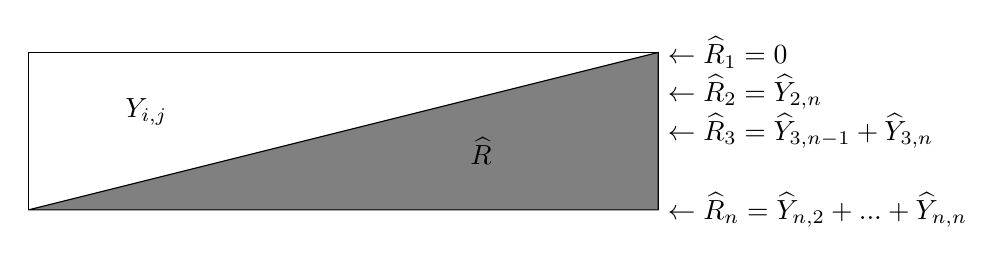
\begin{tikzpicture}
\draw (0,0) rectangle +(8,2);
\draw [fill = gray] (0,0) --(8,2) -- (8,0) -- (0,0);
\node at (1.5,1.25) {$Y_{i,j}$};
\node at (5.75,0.75) {$\widehat{R}$};
\node [right] at (8,2) {$\leftarrow\widehat{R}_1 = 0$};
\node [right] at (8,1.5) {$\leftarrow\widehat{R}_2 = \widehat{Y}_{2,n}$};
\node [right] at (8,1) {$\leftarrow\widehat{R}_3 = \widehat{Y}_{3,n-1} + \widehat{Y}_{3,n}$};
\node [right] at (8,0) {$\leftarrow\widehat{R}_n = \widehat{Y}_{n,2} + ... + \widehat{Y}_{n,n}$};
\end{tikzpicture}
\begin{align*}
\widehat{R}= \sum_{i=1}^{n} \widehat{R}_i
\end{align*}

\begin{align*}
\widehat{Y}_{2,n} &= e^{\widehat{\mu} + \widehat{\alpha}_2 + \widehat{\beta}_n} \\
\widehat{Y}_{3,n-1} &= e^{\widehat{\mu} + \widehat{\alpha}_3 + \widehat{\beta}_{n-1}} \\
\widehat{Y}_{3,n} &= e^{\widehat{\mu} + \widehat{\alpha}_3 + \widehat{\beta}_n} \\
\end{align*}

\end{itemize}

\begin{align*}
\widehat{Y}_{2,n} &= E \Bigg[ e^{\widehat{\mu} + \widehat{\alpha}_2 + \widehat{\beta}_n} \Bigg] \\
&\neq e^{E[\widehat{\mu}] + E[\widehat{\alpha}_2] + E[\widehat{\beta}_n]} \\
\end{align*}
Car $ E[g(X_1,...,X_n)]$ n'égale pas toujours égale à $g(E[X_1],...,E[X_n])$.

\subsection*{Théorème}
Soit $Y = g(X_1,...,X_n)$; une statistique fonction de la $v.a$ $X_1,...,X_n$. En développant la fonction $g(\bullet)$ en série de Taylor multidimensionnelle, et en tronquant après l'ordre 2, on trouve que
\begin{equation}
\label{eq:E[y]}
E[y] \approx g(E[X_1],...,E[X_n]) + \frac{1}{2} \sum_{i=1}^{n} \sum_{j=1}^{n} \frac{\partial^2 g(E[X_1],...,E[X_n])}{\partial X_i \partial X_j} \times \text{Cov}(X_i, X_j) 
\end{equation}
\begin{equation}
\label{eq:Var[y]}
\text{Var}(Y) \approx \sum_{i=1}^{n} \sum_{j=1}^{n} \Bigg( \frac{\partial}{\partial x_i} g(E[X_1],...,E[X_n]) \Bigg) \Bigg( \frac{\partial}{\partial x_j} g(E[X_1],...,E[X_n]) \Bigg) \times \text{Cov}(X_i, X_j)
\end{equation}

\subsubsection*{Exemple}
À partir des équations \ref{eq:E[y]} et \ref{eq:Var[y]} et en posant n = 5, on développe les équations suivantes :
\begin{align*}
\widehat{R}_3 &= \widehat{Y}_{3,4} + \widehat{Y}_{3,5} \\
&= e^{\widehat{\mu} + \widehat{\alpha}_3 + \widehat{\beta}_4} +  e^{\widehat{\mu} + \widehat{\alpha}_3 + \widehat{\beta}_5} \\
&= g(\widehat{\mu}, \widehat{\alpha}_3, \widehat{\beta}_4, \widehat{\beta}_5)
\end{align*}

On développe l'expression de l'espérance de $\widehat{R}_3$
\begin{align*}
E[\widehat{R}_3] & \cong e^{\widehat{\mu} + \widehat{\alpha}_3 + \widehat{\beta}_4} +  e^{\widehat{\mu} + \widehat{\alpha}_3 + \widehat{\beta}_5} \\
& + \frac{1}{2} \Bigg( \Big[ e^{\widehat{\mu} + \widehat{\alpha}_3 + \widehat{\beta}_4} +  e^{\widehat{\mu} + \widehat{\alpha}_3 + \widehat{\beta}_5} \Big] \text{Var}(\widehat{\mu}) \\
& + 2 \Big[ e^{\widehat{\mu} + \widehat{\alpha}_3 + \widehat{\beta}_4} +  e^{\widehat{\mu} + \widehat{\alpha}_3 + \widehat{\beta}_5} \Big] \times \text{Cov}(\widehat{\mu}, \widehat{\alpha}_3) \\
& + 2 \Big[ e^{\widehat{\mu} + \widehat{\alpha}_3 + \widehat{\beta}_4}  \Big] \times \text{Cov}(\widehat{\mu}, \widehat{\beta}_4)\\
& + 2 \Big[ e^{\widehat{\mu} + \widehat{\alpha}_3 + \widehat{\beta}_5}  \Big] \times \text{Cov}(\widehat{\mu}, \widehat{\beta}_5)\\
& + \Big[ e^{\widehat{\mu} + \widehat{\alpha}_3 + \widehat{\beta}_4} +  e^{\widehat{\mu} + \widehat{\alpha}_3 + \widehat{\beta}_5} \Big] \times \text{Cov}(\widehat{\alpha}_3, \widehat{\alpha}_3) \\
& + 2 \Big[ e^{\widehat{\mu} + \widehat{\alpha}_3 + \widehat{\beta}_4}  \Big] \times \text{Cov}(\widehat{\alpha}_3, \widehat{\beta}_4)\\
& + 2 \Big[ e^{\widehat{\mu} + \widehat{\alpha}_3 + \widehat{\beta}_5}  \Big] \times \text{Cov}(\widehat{\alpha}_3, \widehat{\beta}_5)\\
& + \Big[ e^{\widehat{\mu} + \widehat{\alpha}_3 + \widehat{\beta}_4}  \Big] \times \text{Var}(\widehat{\beta}_4)\\
& + 2 \Big[ 0 \Big] \times \text{Cov}(\widehat{\beta}_4, \widehat{\beta}_5)\\
& + 2 \Big[ e^{\widehat{\mu} + \widehat{\alpha}_3 + \widehat{\beta}_5}  \Big] \times \text{Var}(\widehat{\beta}_5) \Bigg)
\end{align*}

On développe l'expression de la variance de $\widehat{R}_3$
\begin{align*}
\text{Var}(\widehat{R}_3) & = \Bigg(  e^{\widehat{\mu} + \widehat{\alpha}_3 + \widehat{\beta}_4} +  e^{\widehat{\mu} + \widehat{\alpha}_3 + \widehat{\beta}_5}\Bigg)^2 \times \text{Var}(\widehat{\mu}) \\
& + 2 \Bigg( e^{\widehat{\mu} + \widehat{\alpha}_3 + \widehat{\beta}_4} +  e^{\widehat{\mu} + \widehat{\alpha}_3 + \widehat{\beta}_5} \Bigg)^2 \text{Cov}(\widehat{\mu}, \widehat{\alpha}_3) \\
& + 2 \Bigg( e^{\widehat{\mu} + \widehat{\alpha}_3 + \widehat{\beta}_4} +  e^{\widehat{\mu} + \widehat{\alpha}_3 + \widehat{\beta}_5} \Bigg) \Bigg( e^{\widehat{\mu} + \widehat{\alpha}_3 + \widehat{\beta}_4} \Bigg)  \times \text{Cov}(\widehat{\mu}, \widehat{\beta}_4) \\
& + 2 \Bigg( e^{\widehat{\mu} + \widehat{\alpha}_3 + \widehat{\beta}_4} +  e^{\widehat{\mu} + \widehat{\alpha}_3 + \widehat{\beta}_5} \Bigg) \Bigg( e^{\widehat{\mu} + \widehat{\alpha}_3 + \widehat{\beta}_5} \Bigg)  \times \text{Cov}(\widehat{\mu}, \widehat{\beta}_5) \\
& + \Bigg( e^{\widehat{\mu} + \widehat{\alpha}_3 + \widehat{\beta}_4} + e^{\widehat{\mu} + \widehat{\alpha}_3 + \widehat{\beta}_5}  \Bigg)^2 \times \text{Var}(\widehat{\alpha}_3)\\
& + 2 \Bigg( e^{\widehat{\mu} + \widehat{\alpha}_3 + \widehat{\beta}_4} +  e^{\widehat{\mu} + \widehat{\alpha}_3 + \widehat{\beta}_5} \Bigg) \Bigg( e^{\widehat{\mu} + \widehat{\alpha}_3 + \widehat{\beta}_4} \Bigg)  \times \text{Cov}(\widehat{\alpha}_3, \widehat{\beta}_4) \\
& + 2 \Bigg( e^{\widehat{\mu} + \widehat{\alpha}_3 + \widehat{\beta}_4} +  e^{\widehat{\mu} + \widehat{\alpha}_3 + \widehat{\beta}_5} \Bigg) \Bigg( e^{\widehat{\mu} + \widehat{\alpha}_3 + \widehat{\beta}_5} \Bigg)  \times \text{Cov}(\widehat{\alpha}_3, \widehat{\beta}_5) \\
& + \Bigg( e^{\widehat{\mu} + \widehat{\alpha}_3 + \widehat{\beta}_4}  \Bigg)^2 \times \text{Var}(\widehat{\beta}_4)\\
& + 2 \Bigg( e^{\widehat{\mu} + \widehat{\alpha}_3 + \widehat{\beta}_4} +  e^{\widehat{\mu} + \widehat{\alpha}_3 + \widehat{\beta}_5} \Bigg) \times \text{Cov}(\widehat{\beta}_4, \widehat{\beta}_5)\\
& + \Bigg( e^{\widehat{\mu} + \widehat{\alpha}_3 + \widehat{\beta}_5}  \Bigg)^2 \times \text{Var}(\widehat{\beta}_5)
\end{align*}

\subsection*{Cas de la loi Poisson}
Dans ce cas, on suppose que $Y_{i,j} \sim Poisson(\mu_{i,j})$ où $\mu_{i,j} = E[Y_{i,j}] = \text{Var}(Y_{i,j})$ et $\mu_{i,j} = e^{\mu + \alpha_i + \beta_j}$ avec $\alpha_1 = \beta_1 = 0$.
Alors, 
\begin{align*}
\phi(\Theta) &= \sum_{i, j \in \triangleleft} \text{ln} \big(f_{Y_{i,j}}(y_{i,j}) \big) \\
&= \sum_{i, j \in \triangleleft} \text{ln} \Bigg( \frac{e^{-\mu_{i,j}} \mu_{i,j}^{y_{i,j}}}{\fact{ y_{i,j}}} \Bigg) \\
&= \sum_{i, j \in \triangleleft} \Bigg( y_{i,j} \text{ln}(\mu_{i,j}) -\mu_{i,j} - \text{ln}(\fact{ y_{i,j}}) \Bigg) \\
\end{align*}

\subsection*{Log-Vraisemblance proportionnelle}
\begin{align*}
\phi(\Theta) &\simeq \sum_{i, j \in \triangleleft} \Bigg( y_{i,j} \text{ln}(\mu_{i,j}) -\mu_{i,j} \Bigg) \\
&= \sum_{i, j \in \triangleleft} \Bigg( y_{i,j} (\mu + \alpha_i + \beta_j) - e^{\mu + \alpha_i + \beta_j} \Bigg) \\
\end{align*}

En pratique, il est impossible de trouver les paramètres tels que $( \widehat{\mu}, \widehat{\alpha_2}, ..., \widehat{\alpha_n}, \widehat{\beta_1},..., \widehat{\beta_n})$ qui maximisent $\phi(\Theta)$ de manière exacte. On utilise donc l'algorithme de  \href{https://fr.wikipedia.org/wiki/Méthode_de_Newton}{Newton-Raphson}.

\begin{align*}
\Theta =
\begin{bmatrix} 
\mu \\
\alpha_2 \\
\vdots \\
\alpha_n \\
\beta_2 \\
\vdots \\
\beta_n \\
\end{bmatrix}
\end{align*}

Avec la méthode de Newton-Raphson : $\Theta^{(i+1)} = \Theta^{(i)} + I(\Theta^{(i)})^{-1}S(\Theta^{(i)})$
Rappel du cours de modèle linéaire : Dans le cas Poisson, on a trouvé que:
$$ S(\Theta) = \mathbb{X}^T \mathbb{W} \text{ ; Où } \mathbb{W} = \mathbb{Y} - \widehat{\mathbb{Y}} $$

De plus, on a
$$
I(\Theta) = \mathbb{X}^\intercal \mathbb{H} \mathbb{X}
$$


\begin{align*}
\mathbb{H} =
\begin{bmatrix} 
e^{X_1 \beta} & \cdots & 0 & \cdots & 0 \\
0  & e^{X_2 \beta} & 0 & \cdots & 0 \\
\vdots & \cdots & \ddots & \cdots & \vdots\\
0 & \cdots & 0 & e^{X_{n-1} \beta} & 0\\
0 & \cdots & 0 & \cdots & e^{X_n \beta}\\
\end{bmatrix}
\end{align*}

\subsubsection*{Remarque}
Dans les formules précédentes de $S(\Theta)$ et $I(\Theta)$; on utilise la formulation sur les GLM acquise dans le cours de modèle linéaire (ACT-2003), soit
$$
Y_{i,j} \sim \text{Poisson}(e^{\mu + \alpha_i + \beta_i}) \sim \text{Poisson}(e^{\mathbb{X} \utilde{\beta}})
$$
Où,
\begin{align*}
\utilde{\beta}=
\begin{bmatrix} 
\beta_0 \\
\beta_1 \\
\vdots \\
\beta_n \\
\end{bmatrix}
\end{align*}

\subsubsection*{Exemple}
Si n = 5, on obtient
\begin{align*}
X_{i,0} &= 1 \\
X_{i,1} &= 1\lbrace i = 2 \rbrace     & X_{i,5} &= 1\lbrace j = 2 \rbrace\\
X_{i,2} &= 1\lbrace i = 3 \rbrace     & X_{i,6} &= 1\lbrace j = 3 \rbrace\\
X_{i,3} &= 1\lbrace i = 4 \rbrace     & X_{i,7} &= 1\lbrace j = 4 \rbrace\\
X_{i,4} &= 1\lbrace i = 5 \rbrace     & X_{i,8} &= 1\lbrace j = 5 \rbrace\\
\end{align*}

\newpage
On exprime les données dans la table suivante:

\begin{center}
\begin{tabular}{|c|c|c|c|c|c|c|c|}
  \hline
   i & j & $Y_{i,j}$ & $X_{i,0}$  & $X_{i,1}$ & $X_{i,2}$ & $\ldots$ & $X_{i,8}$\\
  \hline
  1 & 1 & $\vdots$ & 1 & 1 & 0 & $\cdots$ & 0\\
  1 & 2 & $\vdots$ & 1 & 1 & 0 & $\cdots$ & 0\\
  1 & 3 & $\vdots$ & 1 & 1 & 0 & $\cdots$ & 0\\
  1 & 4 & $\vdots$ & 1 & 1 & 0 & $\cdots$ & 0\\
  1 & 5 & $\vdots$ & 1 & 1 & 0 & $\cdots$ & 1\\
  2 & 1 & $\vdots$ & 1 & 0 & 1 & $\cdots$ & 0\\
  2 & 2 & $\vdots$ & 1 & 0 & 1 & $\cdots$ & 0\\
  2 & 3 & $\vdots$ & 1 & 0 & 1 & $\cdots$ & 0\\
  2 & 4 & $\vdots$ & 1 & 0 & 1 & $\cdots$ & 0\\
  $\vdots$ & $\vdots$ & $\vdots$ & 1 & 0 & 0 & $\vdots$ & $\vdots$ \\
  4 & 1 & $\vdots$ & 1 & 0 & 0 & $\cdots$ & $\vdots$ \\
  4 & 2 & $\vdots$ & 1 & 0 & 0 & $\cdots$ & $\vdots$ \\
  5 & 1 & $\vdots$ & 1 & 0 & 0 & $\cdots$ & $\vdots$ \\
  \hline
\end{tabular}

\end{center}
\subsection*{Suite de l'exemple Excel avec n = 5}
\begin{align*}
\widehat{R} &= 0 \\
&+ \widehat{Y}_{2,5} \\
&+ \widehat{Y}_{3,4} + \widehat{Y}_{3,5} \\
&+ \widehat{Y}_{4,3} + \widehat{Y}_{4,4} + \widehat{Y}_{4,5} \\
&+ \widehat{Y}_{5,2} + \widehat{Y}_{5,3} + \widehat{Y}_{5,4} +  \widehat{Y}_{5,5}\\
\end{align*}

\newpage

On définit $\mathbb{X}^*$ comme suit

\begin{align*}
\mathbb{X}^* =
\begin{bmatrix} 
X^*_0 \\
X^*_1 \\
X^*_2 \\
X^*_3 \\
X^*_4 \\
X^*_5 \\
X^*_6 \\
X^*_7 \\
X^*_8 \\
X^*_9 \\
X^*_{10} \\
\end{bmatrix}
=
\bordermatrix { 
& \mu  &\alpha_2 &\alpha_3 &\alpha_4 & \alpha_5  & \beta_2 & \beta_3 & \beta_4 & \beta_5 \cr 
& 1 & 1 & 0 & 0 & 0 & 0 & 0 & 0 & 1 \cr 
& 1 & 0 & 1 & 0 & 0 & 0 & 0 & 1 & 0 \cr 
& 1 & 0 & 1 & 0 & 0 & 0 & 0 & 0 & 1 \cr 
& 1 & 0 & 0 & 1 & 0 & 0 & 1 & 0 & 0 \cr 
& 1 & 0 & 0 & 1 & 0 & 0 & 0 & 1 & 0 \cr 
& 1 & 0 & 0 & 1 & 0 & 0 & 0 & 0 & 1 \cr 
& 1 & 0 & 0 & 0 & 1 & 1 & 0 & 0 & 0 \cr 
& 1 & 0 & 0 & 0 & 1 & 0 & 1 & 0 & 0 \cr 
& 1 & 0 & 0 & 0 & 1 & 0 & 0 & 1 & 0 \cr 
& 1 & 0 & 0 & 0 & 1 & 0 & 0 & 0 & 1 \cr 
}
\end{align*}


\begin{align*}
\widehat{R} &= e^{X_1^*\widehat{\beta}} + e^{X_2^*\widehat{\beta}} + ... + e^{X_{10}^*\widehat{\beta}} \\
&= g(\beta_0, \beta_1, ..., \beta_{10})
\end{align*}
On obtient ainsi 
\begin{equation}
E[\widehat{R}] = g(\utilde{\widehat{\beta}}) + \frac{1}{2} \sum_{i=0}^{8} \sum_{j=0}^{8} \Bigg( \frac{\partial^2 \widehat{R}}{\partial \utilde{\beta}^2} \Bigg)_{i+1,j+1} \times I^{-1}(\utilde{\widehat{\beta}})_{i+1,j+1}
\end{equation}

Où 
\begin{align*}
\frac{\partial^2 \widehat{R}}{\partial \utilde{\widehat{\beta}}^2} &= [X^*_1]_{i+1} [X^*_1]_{j+1} \times e^{X_1 \utilde{\widehat{\beta}}} + \cdots + [X^*_{10}]_{i+1} [X^*_{10}]_{j+1} \times e^{X_{10}\utilde{\widehat{\beta}}} \\
&= (\mathbb{X}^*)^\intercal \mathbb{W}\mathbb{X}^*
\end{align*}
Où
\begin{align*}
\mathbb{W} = 
\begin{bmatrix} 
e^{X_{1}\utilde{\widehat{\beta}}} & 0 & \cdots & 0 \\
0 & e^{X_{2}\utilde{\widehat{\beta}}}  & \cdots & 0\\
\vdots & \vdots & \ddots & \vdots \\
0 & \cdots & e^{X_{9}\utilde{\widehat{\beta}}} & 0\\
0 & \cdots & 0 & e^{X_{10}\utilde{\widehat{\beta}}} \\
\end{bmatrix}
\end{align*}
Pour la variance de $\widehat{R}$, on obtient
\begin{equation}
\text{Var}(\widehat{R}) = \sum_{i=0}^{8} \sum_{j=0}^{8} \Bigg( \frac{\partial \widehat{R}}{\partial \utilde{\beta}} \Bigg)_{i+1} \times I^{-1}(\utilde{\widehat{\beta}})_{i+1,j+1} \Bigg( \frac{\partial \widehat{R}}{\partial \utilde{\beta}} \Bigg)_{j+1}
\end{equation}
Qu'on peut réécrire en vecteur de la façon suivante,
\begin{equation}
\label{eq:GLM:mat}
\text{Var}(\widehat{R}) = \Bigg( \frac{\partial \widehat{\mathbb{R}}}{\partial \utilde{\beta}} \Bigg)^\intercal I^{-1}(\utilde{\widehat{\beta}}) \Bigg( \frac{\partial \widehat{\mathbb{R}}}{\partial \utilde{\beta}} \Bigg)
\end{equation}

\subsubsection*{Note:}
\begin{align*}
\Bigg( \frac{\partial \widehat{\mathbb{R}}}{\partial \utilde{\beta}} \Bigg) &= [X^*_1] \times e^{X_1 \utilde{\widehat{\beta}}} + \cdots + [X^*_{10}] \times e^{X_{10}\utilde{\widehat{\beta}}} \\
&= (\mathbb{X}^*)^\intercal \mathbb{M}
\end{align*}
Où 
\begin{align*}
\mathbb{M} =
\begin{bmatrix} 
e^{X_1^*\utilde{\beta}} \\
e^{X_2^*\utilde{\beta}}  \\
e^{X_3^*\utilde{\beta}}  \\
e^{X_4^*\utilde{\beta}}  \\
\vdots \\
e^{X_{10}^*\utilde{\beta}} \\
\end{bmatrix}
\end{align*}

Ce qui permet de redéfinir l'équation \ref{eq:GLM:mat} de la façon suivante
\begin{align*}
\text{Var}(\widehat{R}) &= \big( (\mathbb{X}^*)^\intercal \mathbb{M} \big)^\intercal \times I^{-1}(\utilde{\widehat{\beta}}) \times \big( (\mathbb{X}^*)^\intercal \mathbb{M} \big) \\
&= \big( (\mathbb{X}^*)^\intercal \mathbb{\widehat{Y}} \big)^\intercal \times I^{-1}(\utilde{\widehat{\beta}}) \times \big( (\mathbb{X}^*)^\intercal \mathbb{\widehat{Y}} \big)
\end{align*}
Où $\mathbb{\widehat{Y}}$ correspond à la matrice des valeurs des incrémentations estimées.


\subsection*{Tests d'hypothèses avec les GLM}
$H_0$ : Un \textit{sous-modèle} de $M_1$ (noté $M_0$) est acceptable. \newline
$H_1$ : Il est nécessaire d'utiliser le modèle \textit{complet} (noté $M_1$)

Pour tester $H_0$ contre $H_1$, on obtient la statistique 
\begin{equation}
\label{eq:chisquare}
\chi_{obs}^2 = 2 \times \Big( \ell(H_1) - \ell(H_0) \Big)
\end{equation}
Et on rejette $H_0$ au niveau de confiance $100 \times (1 - \alpha) \%$ si \footnote{Où $\Xi$ corresponds au nombre de paramètres.}
\begin{equation}
\label{eq:test:chi}
\chi_{obs}^2 \geq \chi_{\alpha}^2\Big( \text{Nombre de paramètres($\Xi$) de ($M_1$) - Nombre de paramètres($\Xi$) de ($M_0$)} \Big)
\end{equation}


\subsubsection*{Exemple}
Tableau des données : \\
\begin{center}
\begin{tabular}{|c|c|c|c|c|c|}
  \hline
   i / j & 1 & 2  & 3 & 4 \\
  \hline
  1 & 100 & 48 & 23 & 10 \\
  2 & 115 & 55 & 27 &   \\
  3 & 115 & 56 & &   \\
  4 & 115 &  &  &  \\
  \hline
\end{tabular}
\end{center}
\bigskip

\begin{itemize}
\item[A)] 
\begin{align*}
E[Y_{i,j}] &= e^{\mu + \alpha_i + \beta_j} \text{; } \alpha_1 = \beta_1 = 0 \\
\widehat{\mu} &= 4.60 \\
\Xi &= 7 \\
\ell(\widehat{\beta}) & = 2249.283 \\
\end{align*} 
\begin{center}
\begin{tabular}{|c|c|c|}
  \hline
   i / j & 1 & 2\\ 
  \hline
  1 & $\phi$ & $\phi$  \\
  2 & 0.14 & -0.73    \\
  3 & 0.15 & -1.46    \\
  4 & 0.14 &  -2.30  \\
  \hline
\end{tabular}
\end{center}
\bigskip

\item[B)] 
\begin{align*}
E[Y_{i,j}] &= e^{\mu + \alpha_i + \beta \times (j-1)} \text{; } \alpha_1 = 0 \\
\widehat{\mu} &= 4.60 \\
\widehat{\beta} &= -0.74 \\
\Xi &= 5 \\
\ell(\widehat{\beta}) & = 2249.283 \\
\widehat{\alpha}_2 &= 0.15 \\
\widehat{\alpha}_3 &= 0.15 \\
\widehat{\alpha}_4 &= 0.14 \\
\end{align*} 
\subsubsection*{Test}
À l'aide de l'équation \ref{eq:chisquare} on effectue le test d'hypothèse suivant \newline
$H_0$ : Linear developpment $\beta_j = \beta \times (j-1)$ \newline
$H_1$ :  No linear development
\begin{align*}
\chi_{obs}^2 &= 2 \times \Big( 2249.283 - 2248.234 \Big) \\
&= 0.098087 \\
\chi_{0.05}^2(7 - 5) &= 5.99 \\
\end{align*}
Pour rejeter $H_0$, on doit satisfaire l'équation \ref{eq:test:chi},
\begin{align*}
\chi_{obs}^2 &\geq \chi_{\alpha}^2\Big( \Xi (M_1) - \Xi (M_0) \Big) \\
0.098087 &\overset{?}{\geq} 5.99 \\
\end{align*}
On ne peut pas rejeter $H_0$.
\bigskip

\item[C)]
\begin{align*}
E[Y_{i,j}] &= e^{\mu + \alpha\times(i-1) + \beta \times (j-1)} \\
\widehat{\mu} &= 4.64 \\
\widehat{\alpha} &= 0.05 \\
\widehat{\beta} &= -0.73 \\
\Xi &= 3 \\
\ell(\widehat{\beta}, \widehat{\alpha}, \widehat{\mu}) & = 2248.644 \\
\end{align*} 
\subsubsection*{Test}
$H_0$ : Linear trend and developpment ( $e^{\mu + \alpha(i-1) + \beta \times (j-1)}$) \newline
$H_1$ : $H_0$ is false ( $e^{\mu + \alpha_i + \beta_j}$)
\begin{align*}
\chi_{obs}^2 &= 2 \times \Big( 2249.283 - 2248.664 \Big) \\
&= 1.024 \\
\chi_{0.05}^2(7 - 3) &= 9.488 \\
\end{align*}

Pour rejeter $H_0$, on doit satisfaire l'équation \ref{eq:test:chi},
\begin{align*}
\chi_{obs}^2 &\geq \chi_{\alpha}^2\Big( \Xi (M_1) - \Xi (M_0) \Big) \\
1.024 &\overset{?}{\geq} 9.488\\
\end{align*}
On ne peut pas rejeter $H_0$.
\bigskip

\subsubsection*{Alternative au test d'hypothèse}
$H_0$ : Linear trend and developpment ( $e^{\mu + \alpha(i-1) + \beta \times (j-1)}$) \newline
$H_1$ : $H_0$ is false ( $e^{\mu + \alpha_i + \beta \times (j-i)}$)

\bigskip
\item[D)]
On sait qu'il y a eu une nouvelle loi sur le règlement des sinistres à partir de l'année de calendrier 3. $I_{i,j}$ = indicateur de nouvelle loi à i, j.

\begin{center}
\begin{tabular}{|c|c|c|c|c|}
  \hline
   i / j & 1 & 2 & 3 & 4\\ 
  \hline
  1 & 0 & 0 & 1 & 1  \\
  2 & 0 & 1 & 1 &  \\
  3 & 1 & 1 & &   \\
  4 & 1 &  &  &  \\
  \hline
\end{tabular}
\end{center}
\bigskip
\begin{align*}
E[Y_{i,j}] &= e^{\mu + \alpha\times(i-1) + \beta \times (j-1)} + \alpha I_{i,j} \\
\end{align*}
Pour tester si la nouvelle loi a un impact sur le développement, on utilise le $H_0$ suivant
\begin{align*}
H_0 &= e^{\mu + \alpha\times(i-1) + \beta \times (j-1)} \\
\widehat{\mu} &= 4.64 \\
\widehat{\alpha} &= 0.05 \\
\widehat{\beta} &= -0.73 \\
\Xi &= 3 \\
\ell(\widehat{\beta}, \widehat{\alpha}, \widehat{\mu}, \widehat{\alpha}) & = 2248.644 \\
\end{align*}
et le $H_1$ suivant
\begin{align*}
H_1 &= e^{\mu + \alpha\times(i-1) + \beta \times (j-1) + \alpha I_{i,j}} \\
\widehat{\mu} &= 4.64 \\
\widehat{\alpha} &= 0.05 \\
\widehat{\beta} &= -0.73 \\
\widehat{\alpha} &= -001644 \\
\Xi &= 4 \\
\ell(\widehat{\beta}, \widehat{\alpha}, \widehat{\mu}, \widehat{\alpha}) & = 2248.649 \\
\end{align*}
\subsubsection*{Test}
En utilisant les hypothèses $H_0$ et $H_1$ précédentes,
\begin{align*}
\chi_{obs}^2 &= 2 \times \Big( 2248.649-2248.644 \Big) \\
&= 0.009305 \\
\chi_{0.05}^2(4 - 3) &= 3.84 \\
\end{align*}
Pour rejeter $H_0$, on doit satisfaire l'équation \ref{eq:test:chi},
\begin{align*}
\chi_{obs}^2 &\geq \chi_{\alpha}^2\Big( \Xi (M_1) - \Xi (M_0) \Big) \\
0.009305 &\overset{?}{\geq} 3.84\\
\end{align*}
On ne peut pas rejeter $H_0$.
\bigskip
\end{itemize}

\section{Méthode de réserve IARD basée sur la théorie de la crédibilité}

\subsubsection*{Rappel sur C-L }
\begin{enumerate}
\item Le modèle est  bon pour les vieilles AA. Il y a beaucoup de données disponibles, autrement dit, d'expérience individuelle est \textit{crédible}.
\item Par contre, il est moins bon pour les AA récentes. Il y a moins de données, autrement dit, l'expérience individuelle est moins volumineuse et donc moins crédible 
\end{enumerate}
L'idée : Accorder plus de crédibilité à C-L si AA vieille, donc on possède beaucoup de données, et de donner plus de crédibilité à B-F si AA récente.

\subsubsection*{Rappel}
\begin{align*}
\widehat{R}_i^{C-L} &= \widehat{C}_{i,n}^{C-L} - C_{i, n-i+1} \\
&= C_{i,n-i+1} \times \Big(\prod_{j=n-i-1}^{n-1} LDF_j \Big) - C_{i,n-i+1}\\
&= C_{i,n-i+1} \times \Big(\prod_{j=n-i-1}^{n-1} LDF_j - 1 \Big) \\
\end{align*}
\begin{align*}
\widehat{R}_i^{B-F} &= \widehat{C}_{i,n}^{B-F} - C_{i, n-i+1} \\
&= PA_i \times LR_i  - C_{i, n-i+1}\\
&= U_i - \frac{U_i}{\prod_{j=n-i-1}^{n-1} LDF_j}\\
&= U_i \Bigg( 1 - \frac{1}{\prod_{j=n-i-1}^{n-1} LDF_j} \Bigg) \text{; posons } \beta_{n-i+1} = \frac{1}{\prod_{j=n-i-1}^{n-1} LDF_j}\\
&= U_i \Bigg( 1 - \beta_{n-i+1} \Bigg) \\
\end{align*}
L'idée est de combiner $\widehat{R}_i^{C-L}$  et $\widehat{R}_i^{B-F}$.

\begin{align*}
\widehat{R}_i^{Cred} &= C_i \widehat{R}_i^{C-L} + (1 - C_i) \widehat{R}_i^{B-F} \\
&= C_i \times C_{i, n-i+1} \Bigg( \prod_{j=n-i-1}^{n-1} LDF_j - 1 \Bigg) + (1 - C_i) U_i (1 - \beta_{n-i+1}) \\
&= C_i \times C_{i, n-i+1} \Bigg( \prod_{j=n-i-1}^{n-1} LDF_j - 1 \Bigg) + (1 - C_i) U_i (1 - \beta_{n-i+1}) \\
&=C_i \times \widehat{C}_{i, n}^{C-L} - C_i C_{i, n-i+1}  + (1 - C_i) U_i - (1 - C_i)U_i (1 - \beta_{n-i+1}) \\
&= [C_i \times \widehat{C}_{i, n}^{C-L} + (1 - C_i) U_i] - \beta_{n-i+1}\Bigg[ \frac{C_i C_{i, n-i+1}}{\beta_{n-i+1} } + (1 - C_i)U_i\Bigg] \\
\end{align*}
On développe $\beta_{n-i+1}$ afin de réduire l'expression précédante,
\begin{align*}
\beta_{n-i+1} &= \frac{1}{\prod_{j=n-i-1}^{n-1} LDF_j} \\
\frac{1}{\beta_{n-i+1}} &= \prod_{j=n-i-1}^{n-1} LDF_j \\
\frac{C_{i, n-i+1}}{\beta_{n-i+1}} &= C_{i, n-i+1} \prod_{j=n-i-1}^{n-1} LDF_j \\
\frac{C_i C_{i, n-i+1}}{\beta_{n-i+1}} &= C_i C_{i, n-i+1} \prod_{j=n-i-1}^{n-1} LDF_j \\
\frac{C_i C_{i, n-i+1}}{\beta_{n-i+1}} &= C_i \widehat{C}_{i, n}^{C-L} \\
\end{align*}
À partir de cette \textit{identité} et de l'expression suivante, on obtient le résultat suivant
\begin{align*}
\widehat{R}_i^{Cred} &= [C_i \times \widehat{C}_{i, n}^{C-L} + (1 - C_i) U_i] - \beta_{n-i+1} \Bigg[ C_i C_{i, n}^{C-L}  + (1 - C_i)U_i \Bigg] \\
&= [C_i \times \widehat{C}_{i, n}^{C-L} + (1 - C_i) U_i] ( 1 - \beta_{n-i+1}) \\
\end{align*}

Que l'on peut réécrire de la façon suivante
\begin{equation}
\widehat{R}_i^{Cred} = \Bigg[C_{i, n - i + 1} + \Bigg(1 - \frac{1}{\prod_{j = n - i + 1}^{n- 1} \widehat{LDF}_j} \Bigg) PA_i \times LR_i \Bigg] \Bigg(1 - \frac{1}{\prod_{j = n - i + 1}^{n- 1} \widehat{LDF}_j} \Bigg) \\
\end{equation}


Au début des années 1980, Benktander et Hovinen ont trouvé le raisonnement suivant :
\begin{itemize}
\item[i)] $U_i (1 - \beta_{n-i+1}) = R_i^{B-F}$
\item[ii)] $\widehat{R}_i^{B-F} = U_i - C_{i,n-i+1} \Rightarrow \widehat{R}_i^{B-F} = U_i^{B-H} - \widehat{C}_{i,n}\beta_{n-i+1}$
\end{itemize}
À partir de i) $\rightarrow$ ii), on obtient le développement suivant
\begin{align*}
\widehat{C}_{i, n}^{B-F} ( 1 - \beta_{n-i+1} )  &= U_i ^{B-H} - \beta_{n-i+1} \widehat{C}_{i, n}^{C-L} \\
U_i ^{B-H} &= \beta_{n-i+1} \widehat{C}_{i, n}^{C-L} + ( 1 - \beta_{n-i+1} )\widehat{C}_{i, n}^{B-F}  \\
\widehat{C}_{i,n}^{B-H} &= \beta_{n-i+1} \widehat{C}_{i, n}^{C-L} + ( 1 - \beta_{n-i+1} )\widehat{C}_{i, n}^{B-F}  \\
\end{align*}
Où $\beta_{n-i+1}$ correspond à $C_i$ et $( 1 - \beta_{n-i+1} )$ correspond à $ 1 - C_i$.
\newline

En conclusion, pour que l'hypothèse de Benktander - Hoviden soit respectée, autrement dit, à la coïncidence  des diagonales du triangle,  il faut que 
\begin{equation}
C_i = \beta_{n-i+1} = \frac{1}{\prod_{j=n-i+1}^{n-1}} = \text{ La proportion de ce qui a été fait}
\end{equation}

\subsubsection*{Remarque}
En pratique, cette méthode est appelée Bornhuetter - Ferguson itérée. \newline
En répétant  m fois ce raisonnement d'itération, on trouve :
\begin{align*}
 \widehat{C}_{i,n}^{B-H} =
     	\left\{
     	\begin{array}{rl}
     	C_{i,n-i+1} + ( 1 - \beta_{n-i+1} )\widehat{C}_{i, n}^{B-H (m-1)} &, \text{si } m \geq 1 \\
		  C_{i,n-i+1} + ( 1 - \beta_{n-i+1} )U_i &, \text{si } m = 0
     	\end{array}
     	\right.
\end{align*}
Où $U_i = PA_i \times LR_i$
\begin{align*}
\widehat{R}_i^{B-H(m)} = \widehat{C}_{i, n}^{B-H (m)} - C_{i,n-i+1}
\end{align*}
\section{Actualisation des réserves IARD}
Il faut se rappeler qu'on actualise selon l'année de calendrier (Calendar Year (CY))

\begin{center}
\begin{tabular}{|c|c|c|c|c|c|c|c|c|c|}
  \hline
   i & 0 & 12 & 24 & 36 & 48 & 72 & 84 & 0  \\
  \hline
  2005 & & & & & & & & \\
  2006 & & & & & & & & \\
  2007 & & & & & & & & \\
  2008 & & & & & & & & 2015 \\
  2009 & & & & & & & 2015 & 2016 \\
  2010 & & & & & & 2015 & 2016 & 2017 \\
  2011 & & & & & 2015 & 2016 & 2017 & 2018 \\
  2012 & & & & 2015 & 2016 & 2017 & 2018 & 2019  \\
  2013 & & & 2015 & 2016 & 2017 & 2018 & 2019 & 2020  \\
  2014 & & 2015 & 2016 & 2017 & 2018 & 2019 & 2020 & 2021  \\
  \hline
\end{tabular}
\end{center}

\subsubsection*{Étapes}
\begin{itemize}
\item[1)] Développer le triangle avec l'une des méthodes vues en classe : C-L, B-F, Mack, GLM ou B-H.
\item[2)] Calculer les sinistres incrémentaux $Y_{i,j}$ dans la partie inférieure du triangle
\item[3)] Sommer les $Y_{i,j}$ de l'étape 2 par année de calendrier (CY)
\item[4)] Actualiser par CY

\begin{center}
\begin{tabular}{|c|c|c|c|c|c|}
  \hline
   CY & $\sum Y_i$ & Duration & Annual yield curve rate & Actualized figure \\
  \hline
  2015 & $CF_{15}$ & 0.5 & 1 \% & $CF_{15} (1 + 0.01)^{-0.5}$ \\
  2016 & $CF_{16}$ & 1.5 & 2 \% &  $CF_{16} (1 + 0.02)^{-1.5}$\\
  $\vdots$ & $\vdots$ & $\vdots$ & $\vdots$ & $\vdots$  \\
  2021 & $CF_{21}$ & 6.5 & 5 \% & $CF_{21} (1 + 0.05)^{-6.5}$  \\
  \hline
\end{tabular}
\end{center}
\bigskip
$ \widehat{R} = \sum \text{Actualized figure}$ 
\\

\textbf{Notes:} Pour simplifier les calculs, on suppose une distribution uniforme [0, 1] des montants de la réserve et on utilise le point milieu pour l'actualisation.
\end{itemize}
